\documentclass[a4paper]{article}
\usepackage{color}
\usepackage[dvips]{graphicx}
\usepackage{multirow}
\usepackage{wrapfig}
\setlength{\hoffset}{-0.5in}\hoffset-0.5in
\setlength{\textwidth}{15cm}
\topmargin = 20pt
\voffset = -20pt
\addtolength{\textheight}{2cm}
\author{Abigail Millward}
\date{8th of November 2017}

%--------------------------------
\usepackage[
    backend=biber,
    style=authoryear,
    dateabbrev=false,
    language=british
    ]{biblatex}
 
\addbibresource{project_pro.bib}

\begin{document}
\thispagestyle{empty}
\null\vskip0.2in%
\begin{center}
\LARGE{{\bf 
Classificaiton of complex stresses in plants using machine learning}}
\end{center}

\vspace{0.5cm}

\begin{center}
{\Large {\bf by}}\\
\mbox{} \\
{\Large {\bf Abigail Baines (CID: 00742373)}}

{\Large Supervisor : Oliver Windram, Imperial College London, o.windram@imperial.ac.uk}
\end{center}

\vspace{1cm}

\begin{center}
\large{\bf{Department of Life Sciences \\ Imperial College London \\
London SL5 7PY \\ United Kingdom}}
\end{center}


\vspace{1cm}

\begin{figure}[!h]
\centering

\includegraphics[scale=0.35]{imperial_crest_colour.jpg}
\end{figure}

\vspace{1cm}

\begin{center}
\large{\bf{Thesis submitted as part of the requirements for the award of the 
MRes in Computational Methods in Ecology and Evolution, Imperial College London, 2017-2018}} 
\vspace{0.5cm}
\large{\bf{

Formatted in the style of frontiers in Plant Science}}
\vspace{0.5cm}
\large{\bf{

Word count: 5455}}

\end{center}


\vspace{2cm}



  
  \begin{abstract}
    Determining the incidence and types of plant stresses has been of interest for many years, particularly
    due to their potential impact on agricultural production. Despite this, current methods
    are very qualitative, and rely on how the researcher interprets the type and extent of 
    the stress. This is not only time consuming, but also makes comparing results 
    from different studies open to speculation about how each researcher identified the stresses.
    With this in mind, our aim for this project is to see whether we can use machine learning
    to classify and quantify plant stress(es) from multi-spectral leaf images. We aim to do this by
    exposing \textit{Arabidopsis thaliana} to a pathogen (\textit{Botrytis cinerea}) and an abiotic stress. We will then subsequently
    monitor their spectral response following the stress exposure to determine what spectral features
    might evolve in the plant leaves to distinguish between the stressed (both multi$-$level and single
    level) and unstressed (control) plants.
    
    \vspace{5mm}
    Keywords: Digital Pathology, Random Forests, Python, Disease detection,
    Multi-spectral features, Machine Learning.
  \end{abstract}
  
  \section{Introduction}
    Recently, the field of digital pathology has exploded; searching
    digital pathology on Web of Science returns over 3,000 hits, and 2013 onwards
    returns over 250 papers per annum. Despite this, plant pathology remains broadly unexplored using this technology.
    
    The study of plant pathology has always received much attention, due to it's link with
    agricultural yield and crop productivity (\cite{donatelli_modelling_2017, waller_endophytic_2005}). 
    Plant pathology is similar to other streams of pathology; susceptibility is the antithesis of 
    resistance, with resistance being that a plant can overcome or exclude pathogenic effects/organisms.
    The cycle of resistance and susceptibility is powered by natural selection; plants become able to attack
    invading pathogens via their immune response, then pathogens evolve so that they can suppress 
    this triggered immunity, resulting in the plants being susceptible to attack once again
    (\cite{lapin_susceptibility_2013, pel_microbial_2013, zheng_coronatine_2012}). Artificial
    selection in plants has routinely been used in agriculture, in order to introduce resistance to specific
    diseases into crops (\cite{dennis_genetic_2008}).
    
    
    Despite the existence of numerous control measures for many crop diseases (\cite{wood_sustainable_1996})
    , those that still manage to impact upon crop production can be devastating 
    (\cite{mccook_global_2006,woodham-smith_great_1962}).This is further complicated by the fact that different pathogen races and variable environmental conditions can radically affect the degree of disease severity (\cite{dangl_plant_2006, suzuki_reactive_2006}).  Past methods in detecting plant disease
    rely on experts simply observing the plant (\cite{singh_detection_2017}); despite the rise in 
    the use of machine learning for classification, many still rely on manual detection in this field. 
    Manual detection, despite being easily applied in the field, is highly qualitative, and therefore
    is subject to interpretation. It is also noted that manual detection cannot quantify the level of disease 
    severity, and it cannot detect low disease severity accurately (\cite{lowe_hyperspectral_2017}). Our 
    project aims to detect presence/ absence of disease, and severity of disease in plants.
    
    The main aim of this project is to use machine learning to classify instances of complex stress 
    exposure in plants (\textit{Arabidopsis thaliana}). We aim to do this by performing 3 fully replicated experiments to
    capture multi-spectral data from different stress exposures. The stresses the plants will be exposed to are UV stress and \textit{Botrytis cinerea}, a necrotrophic fungus that affects many plant species, and has been used widely in plant biology and pest management studies. The data collected will then be
    used to create an image classifier which will subsequently be tested on additional data samples.
    We also aim to build a fully functional web application to allow other pathologists to use this classifier in
    future research. We anticipate that this project will be successful due to previous work done 
    using machine learning and image analysis, and that this project could be vastly influential to other 
    areas utilizing image analysis techniques.
    
    If our project was to be successful, we anticipate that
    it could be used to aid artificial selection, by choosing the most resistant individuals to breed from
    based on quantitative results, and also precision agriculture. If diseases could be identified to 
    specific individuals rather than whole plots, pesticides could be applied more precisely, minimizing costs 
    to the farmers, and also benefiting ecosystems by reducing mass pesticide application.

    
    
	\section{Materials \& Methods}   
	
	The proposed methods are to gather multi-spectral image data from \textit{Arabidopsis thaliana}, with treatments applied as laid out in
	Table 1.
    
    
  \begin{wraptable}{r}{7cm}
  \caption{Treatment types}
  \begin{tabular}{|c|c|c|c|}
  \hline \cline{2-4}
    & \multicolumn{2}{|c|}{UV Treatment}\\
    \hline
    \multirow{2}{8em}{\textit{Botrytis cinerea} treatment} & ++ & +$-$\\
    & $-$+ & $--$\\
    \hline
  \end{tabular}
  \end{wraptable}

	Images will be taken of each treatment type and used to build a classifier to distinguish treatments.
	We will begin by using a simple random forest approach to classify known multi-spectral and texture features within
	the image set. These classifiers will be used to predict object features such as leaves and disease lesions and to
	distinguish these objects across treatments. This approach will allow us to produce single classifiers within each
	experimental replicate and to test its robustness across remaining replicates. We will use quantifiable metrics to
	score disease. These will include but are not limited to, the size of disease lesions between treatments and
	quantitative differences in the colour of leaves. For example the degree of chlorosis can be use to estimate and
	compare levels of disease severity between treatments. In addition to the complex stress trial planned for this
	project we will also process additional image data available from the lab members of diseased plants with different
	genetic backgrounds. In doing so we will look to quantify different levels of disease susceptibility in plants. 
	
	The pipeline outlined above will be written in python, with some code being translated from existing code 
    written in matlab and R. We will also use packages such as opencv and ilastik to further build the pipeline, as well
    as to begin developing the web application.
    
    The pipeline is highly adaptable and broadly applicable to a wide range of pathologies. To make this approach more 
    broadly applicable to the plant pathology community we aim to develop a simple web application that new users
    can use to build classifiers to distinguish and quantify pathologies of their choice.
    
	
	\section{Gantt chart}
	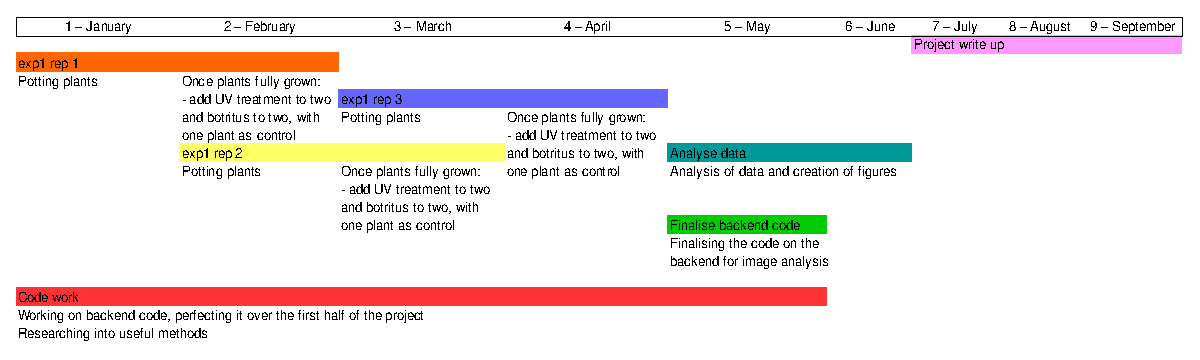
\includegraphics[width =\textwidth]{gantt_chart.eps}
	
	\section{Budget}
	
	The anticipated budget for this project is as follows:
	\vspace{2mm}
	
	$-$ template for frontend webpage $-$ \pounds70
	\vspace{3mm}
	
    $-$ Software and VPN $-$ \pounds60
    \vspace{3mm}
  
    $-$ Backend management system $-$ \pounds80 
    \vspace{3mm}
  
    $-$ Sundries and consumables $-$ for plants \pounds300
    \vspace{3mm}
  
    $-$ Travelling costs $-$ \pounds100
    \vspace{3mm}
  
    $-$ Miscellaneous $-$ \pounds100
    \vspace{2mm}
    
    Supervisor Oliver Windram has seen and accepted budget.
  
  \printbibliography

\end{document}
